% intro.tex:

\chapter{Introduction}
\label{chap:intro}



\section{Trial and error}
\label{chap:intro:design}

Trial and error has been the fundamental method~\cite{cowles2015hypothesis}

\begin{figure}
	\centering
	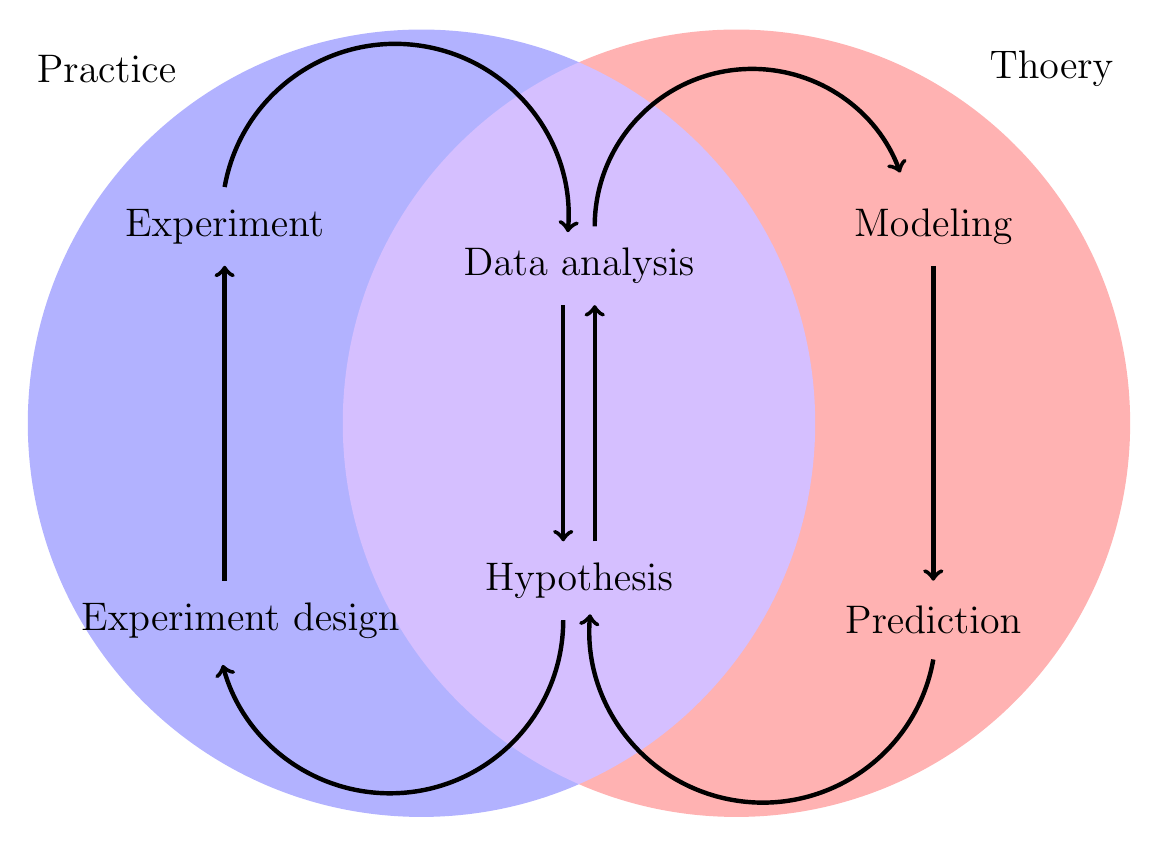
\begin{tikzpicture}
		\begin{scope}[blend group = soft light]
			\fill[blue!30!white] (-2,0) ellipse (5 and 5);
			\fill[red!30!white]  (+2,0) ellipse (5 and 5);
		\end{scope}
		\draw[ultra thick, ->] (0.2,2.5) arc (0:-160:-2);
		\draw[ultra thick, ->] (-4.5,+3) arc (-10:-185:-2.2);
		\draw[ultra thick, ->] (-0.2,-2.5) arc (0:-165:+2.2);
		\draw[ultra thick, ->] (4.5,-3) arc (-10:-185:2.2);
		\draw [ultra thick, ->] (-0.2,+1.5) -- (-0.2,-1.5);
		\draw [ultra thick, ->] (+0.2,-1.5) -- (+0.2,+1.5);
		\draw [ultra thick, ->] (4.5,+2) -- (4.5,-2);
		\draw [ultra thick, ->] (-4.5,-2) -- (-4.5,+2);
		\node at (0,+2)[font=\Large]  {Data analysis};
		\node at (4.5,+2.5)[font=\Large]  {Modeling};
		\node at (4.5,-2.5)[font=\Large]  {Prediction};
		\node at (0,-2)[font=\Large]  {Hypothesis};
		\node at (-4.5,+2.5)[font=\Large]  {Experiment};
		\node at (-4.3,-2.5)[font=\Large]  {Experiment design};
		\node at (-6,4.5)[font=\Large]    {Practice};
		\node at (+6,4.5)[font=\Large]    {Thoery};
	\end{tikzpicture}
	\caption{Theory and practice in engineering and scientific research.}
\end{figure}

